% Slide: Bar Chart Results
\begin{frame}{Tuning Results: Optimal Values vs. Matrix Size}
	
	\begin{figure}
		\centering
		% NOTE: This uses the PGFPlots code from your expts.tex file
		% First bar chart
		\pause 
		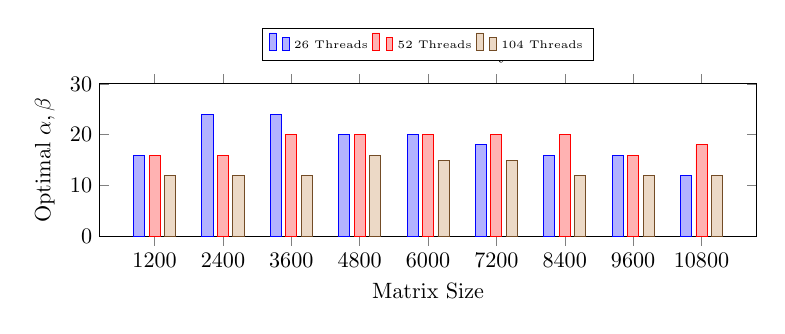
\begin{tikzpicture}[scale=0.8, transform shape]
		  \begin{axis}[
		      title={Without Priority},
		      ybar,
		      bar width=5pt,
		      symbolic x coords={1200,2400,3600,4800,6000,7200,8400,9600,10800},
		      xtick=data,
		      xlabel={Matrix Size},
		      ylabel={Optimal $\alpha, \beta$},
		      legend style={at={(0.5,1.15)}, anchor=south, legend columns=-1, font=\tiny},
		      ymin=0, ymax=30,
		      width=12cm, height=4cm
		      ]
		      \addplot coordinates {(1200,16) (2400,24) (3600,24) (4800,20) (6000,20) (7200,18) (8400,16) (9600,16) (10800,12)};
		      \addplot coordinates {(1200,16) (2400,16) (3600,20) (4800,20) (6000,20) (7200,20) (8400,20) (9600,16) (10800,18)};
		      \addplot coordinates {(1200,12) (2400,12) (3600,12) (4800,16) (6000,15) (7200,15) (8400,12) (9600,12) (10800,12)};
		      \legend{26 Threads, 52 Threads, 104 Threads}
		  \end{axis}
		\end{tikzpicture}
		
		\vspace{4mm}
		\pause 
		% Second bar chart
		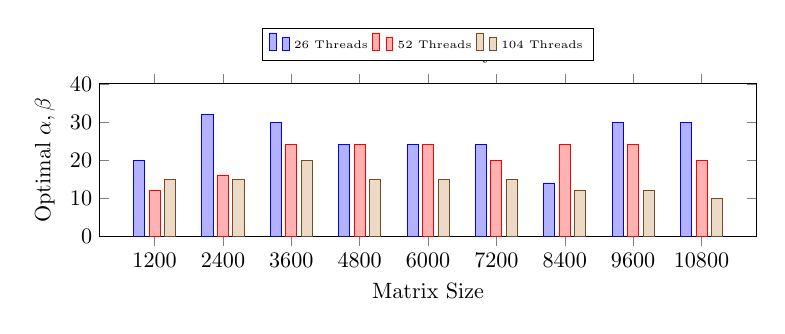
\begin{tikzpicture}[scale=0.8, transform shape]
		  \begin{axis}[
		      title={With Priority},
		      ybar,
		      bar width=5pt,
		      symbolic x coords={1200,2400,3600,4800,6000,7200,8400,9600,10800},
		      xtick=data,
		      xlabel={Matrix Size},
		      ylabel={Optimal $\alpha, \beta$},
		      legend style={at={(0.5,1.15)}, anchor=south, legend columns=-1, font=\tiny},
		      ymin=0, ymax=40,
		      width=12cm, height=4cm
		      ]
		      \addplot coordinates {(1200,20) (2400,32) (3600,30) (4800,24) (6000,24) (7200,24) (8400,14) (9600,30) (10800,30)};
		      \addplot coordinates {(1200,12) (2400,16) (3600,24) (4800,24) (6000,24) (7200,20) (8400,24) (9600,24) (10800,20)};
		      \addplot coordinates {(1200,15) (2400,15) (3600,20) (4800,15) (6000,15) (7200,15) (8400,12) (9600,12) (10800,10)};
		      \legend{26 Threads, 52 Threads, 104 Threads}
		  \end{axis}
		\end{tikzpicture}
	\end{figure}
  
\end{frame}